% !TeX program = pdflatex
% !TeX root = main.tex
% ChkTeX interprets deliberate en dashes, acronym sentence endings,
% caption-label line breaks, and abbreviated table headings as warnings.
% chktex-file 8
% chktex-file 12
% chktex-file 13
% chktex-file 24
\documentclass[11pt]{article}
\usepackage[T1]{fontenc}
\usepackage[utf8]{inputenc}
\usepackage[margin=1in]{geometry}
\usepackage{amsmath}
\usepackage{graphicx}
\usepackage{booktabs}
\usepackage[hidelinks]{hyperref}
\setlength{\parindent}{0pt}
\setlength{\parskip}{0.5\baselineskip}
\setlength{\emergencystretch}{2em}
\title{Clinically Significant Prostate Cancer Classification from T2-Weighted and ADC MRI Patches: An Auditable PROSTATEx Study}
\author{Mohammad Rashid Dubayan\textsuperscript{1,*} \and
Hamid Haj Seyyed Javadi\textsuperscript{1,*} \and
Hasanain Flayyih Hasan\textsuperscript{2,*}}
\date{}
\begin{document}
\maketitle
\begin{center}
\small
\textsuperscript{1}Department of Computer Engineering, Shahed University,\\
Tehran 3319118651, Iran\\
\textsuperscript{2}Department of Cybersecurity, College of Computer Science\\
and Information Technology, Wasit University, Iraq\\[0.5em]
\textsuperscript{*}Correspondence, as listed in the source manuscript:\\
\nolinkurl{mohamed313rashid@gmail.com}; \nolinkurl{4039175003@shahed.ac.ir}\\
\nolinkurl{h.s.javadi@shahed.ac.ir}; \nolinkurl{hasanain.f.h@uowasit.edu.iq}
\end{center}

\begin{abstract}

This study develops and audits a patient-level evaluation pipeline for classifying clinically significant prostate cancer findings from T2-weighted and apparent diffusion coefficient (ADC) magnetic resonance imaging patches in PROSTATEx. A frozen technical-eligibility process retained 306 findings from 191 patients, including 65 clinically significant findings. Spatially corresponding $100\times100$ T2 and ADC patches were evaluated using five fixed outer folds with no patient overlap. Fixed convolutional neural networks (CNNs) were trained on T2, ADC, and paired T2/ADC inputs with three random seeds. Matched classical controls used deterministic intensity-summary features with logistic regression, a radial-basis-function support vector machine, and random forest. Performance was calculated from pooled out-of-fold predictions, with 95\% confidence intervals from 2,000 patient-level bootstrap replicates. Fixed-CNN area under the receiver operating characteristic curve (AUC) values were 0.6086 for T2, 0.6479 for ADC, and 0.6634 for paired T2/ADC. The highest primary AUC was 0.7205 (95\% confidence interval 0.6516--0.7882) for random-forest ADC. In an exploratory paired bootstrap without multiplicity adjustment, this exceeded the modality-matched ADC CNN by 0.0725 AUC (95\% confidence interval 0.0084--0.1397); the other eight modality-matched classical-versus-CNN intervals included zero. Excluding one finding with limited native ADC support did not materially change the results. These findings demonstrate a reproducible prostate MRI benchmarking workflow but do not establish clinical utility, external validity, or a general advantage for CNNs over simpler controls.

\end{abstract}

\textbf{Keywords:} Prostate cancer; magnetic resonance imaging; PROSTATEx; apparent diffusion coefficient; convolutional neural networks; random forest; patient-level validation; reproducibility.

\section{Introduction}\label{sec:1}

Classification of clinically significant prostate cancer from magnetic resonance imaging (MRI) requires both a defensible image-processing pipeline and an evaluation design that prevents information from the same patient appearing on both sides of model assessment. T2-weighted imaging provides anatomical contrast, whereas apparent diffusion coefficient (ADC) images summarize diffusion-sensitive signal behavior; both are incorporated into standardized prostate MRI assessment pathways~\cite{pirads-v21,pirads-pathway}. PROSTATEx provides public prostate MRI studies and finding-level labels that support methodological evaluation of these inputs~\cite{prostatex}. However, the presence of public images and labels does not by itself define which series should be selected, how channels should be spatially paired, or how repeated findings from one patient should be partitioned.

These implementation decisions are especially important for reproducibility. A patient may have multiple studies, series descriptions may be ambiguous, and DICOM volumes may contain geometric irregularities or incomplete physical coverage. T2 and ADC images can also differ in matrix size, orientation, spacing, and slice positions. Patch extraction must therefore operate in patient coordinates rather than by assuming that corresponding array indices represent the same anatomy. Eligibility rules, series selection, boundary handling, and exclusion decisions should be frozen before model outcomes are inspected.

Evaluation design presents a second challenge. Multiple findings from one patient are statistically dependent, so random finding-level splitting can produce optimistic results through patient overlap. Model selection and all learned preprocessing must remain within the training and validation patients, while the outer test fold remains untouched until final prediction. Uncertainty estimates should likewise resample patients rather than individual findings. The class distribution also requires metrics beyond raw accuracy because clinically significant findings form a minority of the retained cohort.

The modeling question in this study is deliberately limited: how do compact fixed convolutional neural networks (CNNs) compare with conventional classifiers when both use the same frozen patients, findings, image channels, and outer folds? Three image inputs are considered: T2 only, ADC only, and paired T2/ADC. The classical controls use deterministic intensity summaries extracted from the same patches and include logistic regression, a radial-basis-function support vector machine, and random forest. Paired input is evaluated rather than assumed to be beneficial, and discrimination, threshold-dependent performance, and calibration are reported separately.

The resulting analysis is an auditable benchmark, not a clinical diagnostic validation. It uses one public cohort, has no external test set, lacks verified ADC physical units, and does not include qualified diagnostic image-quality review or lesion segmentation. The objective is to establish a reproducible technical foundation and quantify the performance of transparent baseline models before considering more complex architectures, augmentation, or optimization strategies. The emphasis on explicit data flow, partitioning, reference-standard limitations, and artifact availability is consistent with reporting priorities in CLAIM and TRIPOD+AI~\cite{claim,tripod-ai}.

\subsection{Contributions}\label{sec:1.1}

\begin{itemize}
\item A hash-audited PROSTATEx retrieval, eligibility, series-selection, and paired-patch extraction workflow with explicit geometric and boundary checks.
\item A frozen five-fold patient-level evaluation design for 306 findings from 191 patients, with model selection separated from outer-fold testing.
\item Matched fixed-CNN and classical baselines for T2, ADC, and paired T2/ADC inputs, supported by complete out-of-fold predictions and run artifacts.
\item Patient-level bootstrap confidence intervals and paired model comparisons that preserve all findings from each resampled patient.
\item A prespecified sensitivity analysis for one finding with limited native ADC support, together with explicit technical and clinical limitations.
\end{itemize}

\subsection{Paper Organization}\label{sec:1.2}

Section~\ref{sec:2} reviews relevant prostate MRI modeling and evaluation considerations. Section~\ref{sec:3} describes cohort construction, paired-patch extraction, patient-level folds, and the CNN and classical baselines. Section~\ref{sec:4} reports out-of-fold performance, sensitivity analyses, paired comparisons, and calibration. Section~\ref{sec:5} discusses the findings and limitations, Section~\ref{sec:6} concludes the study, and Section~\ref{sec:7} identifies priorities for future validation and modeling.

\section{Related Work}\label{sec:2}

\subsection{Public Prostate MRI Benchmarks}\label{sec:2.1}

PROSTATEx was designed as a lesion-level challenge for distinguishing clinically significant from non-significant prostate findings using multiparametric MRI~\cite{prostatex,armato-prostatex}. The challenge provided centralized training and test cohorts and required a continuous likelihood for each test lesion. Across 71 submitted methods, reported test AUCs ranged from 0.45 to 0.87, while differences among the leading methods were not statistically established~\cite{armato-prostatex}. These results illustrate both the feasibility of image-based classification and the uncertainty associated with ranking algorithms on a modest test cohort.

The public release has enabled later methodological studies, but published results are not automatically comparable. Investigators have used different subsets of patients and findings, different MRI sequences, varying levels of manual annotation, and different internal validation procedures. Some studies use the original hidden challenge test set, whereas others perform cross-validation on the released training cohort. A reproducible study must therefore state exactly which cohort, labels, exclusions, and partitioning unit were used rather than treating all PROSTATEx scores as measurements from one common protocol.

The later PI-CAI study illustrates the increasing scale and rigor of prostate MRI AI evaluation. Its consortium trained and externally tested an AI system using 10,207 MRI examinations from 9,129 patients and compared performance with a multinational reader study and multidisciplinary routine practice~\cite{picai-confirmatory}. That confirmatory design is substantially different from the present internal benchmark, but it provides a contemporary reference for the external testing, reader comparison, and prespecified clinical evaluation required for stronger claims.

\subsection{Deep Learning for Finding Classification}\label{sec:2.2}

Mehrtash et al.~\cite{mehrtash-prostatex} developed a 3D CNN for the PROSTATEx task and examined combinations of ADC, high-b-value diffusion imaging, dynamic contrast-enhanced imaging, and zonal information. Their reported challenge-test AUC of 0.80 shows that volumetric CNNs can use multiparametric inputs, but their architecture, sequences, augmentation, and evaluation cohort differ from the two-dimensional T2/ADC patch baselines considered here. Schelb et al.~\cite{schelb-pirads} subsequently compared deep-learning classification with clinical PI-RADS assessment, further demonstrating that algorithmic performance must be interpreted relative to the clinical reading framework and reference standard. Other multi-input studies similarly indicate that sequence choice can materially affect classification, so adding channels should be evaluated empirically rather than assumed to improve performance.

Deep models can learn spatial features directly from image neighborhoods, but this flexibility increases dependence on preprocessing, registration, field of view, and training sample size. Reported performance can also reflect manual lesion localization, prostate masks, anatomical-zone inputs, or additional MRI sequences. The present work intentionally uses small fixed CNNs and recorded finding coordinates so that the data pipeline and evaluation design can be audited independently of a highly optimized architecture.

\subsection{Radiomics and Classical Machine Learning}\label{sec:2.3}

Feature-based approaches remain relevant controls for prostate MRI. Kwon et al.~\cite{kwon-prostatex} extracted intensity and texture measurements from manually outlined structures across T2-weighted, ADC, high-b-value, and dynamic contrast-enhanced inputs. Their random-forest model achieved a challenge-test AUC of 0.82, outperforming their CART and adaptive-LASSO models. This result is not directly comparable with the present study because the feature set, manual contours, modalities, and test protocol differ, but it demonstrates that classical models can be competitive on the same clinical task.

Castillo Tovar et al.~\cite{castillo-validation} compared a deep-learning model with a radiomics approach across several cohorts, scanners, and reference-standard settings. Their validation design emphasizes that performance observed within one center or dataset may not transfer unchanged to external populations. In the present study, deterministic patch summaries and classical classifiers serve as matched controls rather than as a comprehensive radiomics pipeline: they use the same findings, channels, outer folds, and test predictions as the CNN experiments.

\subsection{Multimodal Alignment and Input Definition}\label{sec:2.4}

T2 and diffusion-derived images provide different information and are commonly acquired with different spatial resolutions and slice geometries. Prior PROSTATEx methods have addressed this issue through rigid fusion, resampling, manual contours, or three-dimensional crops~\cite{mehrtash-prostatex,kwon-prostatex}. These choices affect which anatomy is presented to a classifier. A paired-input experiment is therefore meaningful only when both channels are sampled on a documented common physical grid and findings that lack complete support are handled by a prespecified rule.

The present study samples the same patient-coordinate grid in T2 and ADC while retaining the T2 plane orientation. It does not claim deformable registration, calibrated ADC units, or lesion segmentation. This restricted design isolates the predictive value of local stored intensities but cannot determine whether more advanced registration, prostate localization, or lesion-aware inputs would improve performance.

\subsection{Model Selection and Credible Evaluation}\label{sec:2.5}

Cawley and Talbot~\cite{selection-bias} show that model selection can overfit a finite validation set and bias performance estimates when the same information influences both tuning and assessment. This concern is amplified when several findings belong to one patient. Patient-level outer folds, training-only preprocessing, validation-only model selection, and untouched outer-fold prediction are therefore central to credible evaluation. CLAIM and TRIPOD+AI likewise emphasize transparent reporting of data partitions, model-development procedures, performance assessment, and open-science materials~\cite{claim,tripod-ai}.

Confidence intervals and paired comparisons should also respect patient clustering. Resampling individual findings would treat correlated observations as independent and can understate uncertainty. The present work pools one out-of-fold prediction per finding, resamples complete patients for bootstrap intervals, and uses identical resampled patients when comparing models. Even with these safeguards, one public cohort cannot establish external validity or clinical utility.

\section{Materials and Methods}\label{sec:3}

\subsection{Task, Source Data, and Finding Identity}\label{sec:3.1}

The study uses the public PROSTATEx collection~\cite{prostatex}. The prediction unit is a recorded finding rather than a complete MRI examination. Each finding is identified by patient identifier, finding identifier, and the supplied three-dimensional patient-coordinate position. The binary outcome is the recorded \texttt{ClinSig} field, encoded as 1 for clinically significant and 0 for non-significant disease. The task is therefore finding-level classification at a supplied location; it is not lesion detection, segmentation, or whole-examination diagnosis.

The source finding table contained 204 patients and 330 findings. Six patients comprising 10 findings were used repeatedly during pipeline development and were excluded from all reported model fitting and evaluation. One additional patient, ProstateX-0191, lacked the prespecified canonical axial T2 series and was excluded from the paired primary cohort. This left 197 patients and 319 findings planned for paired retrieval. Post-retrieval hard checks excluded six complete patients with 12 findings and one additional finding whose complete grid lay outside the ADC pixel-center bounds, without patient replacement or fold movement. The final technically accepted cohort therefore contained 191 patients and 306 findings, comprising 65 positive and 241 negative findings. Series-selection rules and technical hard checks were frozen before bulk cohort retrieval and before model training. Source contents, eligibility decisions, patches, and modeling outputs were tracked by SHA-256 hashes.

\subsection{Series Selection and Technical Eligibility}\label{sec:3.2}

Candidate T2 series required the normalized description \texttt{t2\_tse\_tra}; candidate ADC series required a normalized description ending in \texttt{\_ADC}. A T2/ADC pair had to belong to the same patient and study. When several eligible pairs remained within a study, a metadata-only ascending order of T2 series number, ADC series number, T2 series UID, and ADC series UID determined the primary pair. Labels, visual appearance, and model performance were not used for series selection. All nonprimary eligible pairs were retained in the audit records. ProstateX-0025 was a frozen multi-study exception: each of its five full finding keys was assigned to the unique study pair whose complete output grid contained that finding, and these geometry-only assignments were fixed before bulk retrieval and modeling.

After DICOM retrieval, each selected series underwent archive, identity, encoding, and geometry checks. These included CRC validation, unique member and SOP-instance identifiers, consistent patient/study/series identities, supported native single-frame pixel encoding, consistent dimensions and spacing, orthonormal in-plane directions, and monotonic regular physical slice steps. T2 and ADC also had to share the audited frame of reference. Findings were rejected if the complete output grid did not lie within both source volumes; clinical padding, extrapolation, or image-based substitution was prohibited.

\subsection{Paired Patch Construction}\label{sec:3.3}

For a finding at patient-coordinate position $\mathbf{p}$, a $100\times100$ grid was constructed parallel to the selected T2 plane. Let $\mathbf{r}$ and $\mathbf{c}$ denote the T2 row and column unit directions. Pixel-center offsets were

\begin{equation}
d_u=\left(u-\frac{99}{2}\right)0.5\ \mathrm{mm},\qquad u=0,\ldots,99,
\end{equation}

and the world coordinate of output pixel $(u,v)$ was

\begin{equation}
\mathbf{q}_{uv}=\mathbf{p}+d_u\mathbf{c}+d_v\mathbf{r}.
\label{eq:patch-grid}
\end{equation}

Thus, both channels were sampled on the same 0.5-mm grid with pixel-center offsets from $-24.75$ to $24.75$ mm. Patient coordinates were transformed to source voxel coordinates using the inverse audited DICOM affine. Trilinear interpolation was applied independently to T2 and ADC. A point outside the source pixel-center bounds by more than $10^{-4}$ voxel caused rejection; smaller numerical overshoot was clipped to the nearest boundary. No clinical padding or clipping was used.

Stored unsigned pixel values were converted to \texttt{float32}. No intensity normalization, modality lookup table, rescale transformation, real-world-value conversion, or ADC-unit conversion was applied during patch construction. The final arrays had shape $2\times100\times100$ per finding. Across all folds, 384 source series contributed to the accepted patch set, and all patch arrays were finite and hash-verified.

\subsection{Technical Quality Control and Sensitivity Finding}\label{sec:3.4}

Automated checks verified bundle CRCs, artifact hashes, finding keys, labels, fold assignments, array shapes, finite values, and complete-grid bounds. A label-hidden display review found no obvious blank-channel or gross resampling problem in 305 of 306 paired patches. One retained finding, ProstateX-0052 finding 1, had limited native ADC signal support and a predominantly zero-valued ADC patch. Under the frozen zero-value policy, the finding remained in every primary analysis and its patient remained in the original fold. A prespecified sensitivity analysis removed only this finding from ADC-only and paired T2/ADC data before constructing all training, validation, and test arrays; the T2-only analysis was unchanged and no replacement finding was introduced.

\subsection{Frozen Patient-Level Folds}\label{sec:3.5}

Patients were assigned once to five outer folds using a deterministic class-aware allocation, and every finding from one patient remained in the same fold. Table~\ref{tab:cohort-folds} summarizes the final accepted cohort. For evaluation cycle $k$, fold $k$ was the test fold, fold $(k+1)\bmod 5$ was the validation fold, and the remaining three folds were used for training. Post-retrieval exclusions were not replaced and no patient was moved after outcomes or model results were inspected.

\begin{table}[htbp]
\centering
\caption{Frozen outer-fold composition of the technically accepted PROSTATEx cohort.}
\label{tab:cohort-folds}
\begin{tabular}{@{}rrrr@{}}
\toprule
\textbf{Outer fold} & \textbf{Findings} & \textbf{ClinSig positive} & \textbf{ClinSig negative} \\
\midrule
0 & 64 & 15 & 49 \\
1 & 57 & 12 & 45 \\
2 & 62 & 13 & 49 \\
3 & 62 & 12 & 50 \\
4 & 61 & 13 & 48 \\
\midrule
Total & 306 & 65 & 241 \\
\bottomrule
\end{tabular}
\end{table}

\subsection{Fixed CNN Baselines}\label{sec:3.6}

Separate CNN configurations used T2 only, ADC only, or paired T2/ADC channels. Within each evaluation cycle, the mean and standard deviation of every selected channel were calculated across training patches and pixels only. The same training statistics standardized the validation and test patches; the minimum permitted standard deviation was $10^{-6}$. No clipping or data augmentation was applied.

The fixed CNN comprised two blocks: $3\times3$ convolution with 16 or 32 output channels, batch normalization, ReLU, and $2\times2$ max pooling. Adaptive global average pooling was followed by flattening, dropout of 0.25, and a linear layer producing one logit. Training used weighted binary cross-entropy, with positive weight equal to the ratio of negative to positive training findings, and Adam with learning rate $10^{-3}$, weight decay $10^{-4}$, and batch size 32. Training continued for at most 100 epochs and stopped after 15 epochs without improvement in validation ROC AUC. The checkpoint with the highest validation AUC was applied once to the outer test fold.

Each fold and modality was trained with seeds 1729, 2718, and 3141. For each finding, the three out-of-fold probabilities were averaged before pooled metrics were calculated. The primary analysis comprised 45 CNN runs; ADC and paired sensitivity analyses added 30 runs, for 75 runs in total.

\subsection{Classical Baselines}\label{sec:3.7}

Classical controls used deterministic features from the same frozen patches. For each channel, a fixed $10\times10$ block partition produced 100 block means and 100 block standard deviations. Ten global summaries were appended: mean, standard deviation, minimum, maximum, the 10th, 25th, 50th, 75th, and 90th percentiles, and the exact-zero fraction. This yielded 210 features per channel and 420 features for paired input. These generic intensity summaries are controls, not a validated radiomics feature set.

Logistic regression used a training-fitted standardizer, class weighting, the \texttt{liblinear} solver, and $C\in\{0.001,0.01,0.1,1,10\}$. The probability-enabled RBF SVM used a training-fitted standardizer, class weighting, $C\in\{0.1,1,10\}$, and $\gamma\in\{\texttt{scale},0.01\}$. Random forest used 500 trees, square-root feature subsampling, balanced-subsample class weighting, maximum depth in $\{\texttt{None},6,12\}$, and minimum leaf size in $\{1,4\}$. Candidate selection maximized validation ROC AUC, with the first candidate in the frozen grid resolving ties. The selected estimator remained fitted only on the three training folds and was evaluated on the outer test fold without refitting on validation data. The nine primary and six sensitivity configurations across five test folds produced 75 runs.

\subsection{Metrics, Uncertainty, and Model Comparisons}\label{sec:3.8}

Reported metrics were ROC AUC, average precision, accuracy, balanced accuracy, sensitivity, specificity, precision, F1 score, and Brier score. Threshold-dependent metrics used a fixed probability threshold of 0.5; ROC AUC and average precision used continuous scores. Metrics were calculated from pooled out-of-fold predictions so that every accepted finding contributed exactly one test prediction per configuration.

Confidence intervals were percentile intervals from 2,000 patient-level bootstrap replicates. Complete patients were sampled with replacement, preserving all findings belonging to each sampled patient. CNN summaries used bootstrap seed 8675309, and classical summaries used seed 97531. Paired differences between primary models used identical sampled patients for both predictions. The primary CNN input comparisons used 10,000 replicates with seed 24681357; modality-matched classical-minus-CNN comparisons used 10,000 replicates with seed 86420. These paired comparisons were exploratory and were not adjusted for multiplicity. An interval containing zero was not interpreted as establishing a difference.

\section{Results}\label{sec:4}

\subsection{Cohort and Artifact Integrity}\label{sec:4.1}

The frozen cohort contained 191 patients and 306 technically accepted findings, with 65 clinically significant and 241 non-significant findings. The five outer folds contained 57--64 findings each and 12--15 positive findings, as shown in Table~\ref{tab:cohort-folds}. All findings from one patient remained in one fold throughout patch extraction, model selection, sensitivity analysis, and testing.

The final paired-patch set used 384 unique source series. All five patch bundles passed CRC and artifact-hash checks; all finding keys, labels, and fold assignments matched the frozen eligibility register; and every array contained finite values. No clinical padding or out-of-bounds clipping was used. The maximum numerical boundary snap was $1.57\times10^{-5}$ voxel, below the prespecified $10^{-4}$-voxel tolerance.

The fixed-CNN archive contained 75 completed runs, including model states, training histories, test predictions, and result files. The classical archive contained 75 completed runs, 75 serialized estimators, 75 candidate-score tables, 75 test-prediction tables, and one run index. Independent recomputation reproduced all summary metrics, and every fold-level prediction table matched its corresponding pooled summary exactly.

\subsection{Fixed CNN Baselines}\label{sec:4.2}

Table~\ref{tab:4} reports three-seed ensemble out-of-fold results for the frozen prostate MRI experiment. The paired T2/ADC model has the highest primary AUC, 0.6634 (patient-bootstrap 95\% CI 0.5923--0.7357), followed by ADC at 0.6479 (0.5745--0.7218) and T2 at 0.6086 (0.5308--0.6822). The overlapping intervals and modest absolute values do not establish superiority of paired inputs. At the fixed 0.5 threshold, ADC has the highest primary accuracy and balanced accuracy, whereas the paired model has higher sensitivity but lower specificity. Thus, the ranking depends on the target metric and threshold.

\begin{table}[htbp]
\centering
\scriptsize
\caption{Exploratory PROSTATEx fixed-CNN results from three-seed averaged out-of-fold predictions. Confidence intervals are based on 2,000 patient-level bootstrap replicates. AP denotes average precision; Bal. Acc. denotes balanced accuracy.}
\label{tab:4}
\resizebox{\linewidth}{!}{%
\begin{tabular}{@{}llrrrrrrr@{}}
\toprule
\textbf{Input} & \textbf{Analysis} & \textbf{$n$} & \textbf{AUC (95\% CI)} & \textbf{AP} & \textbf{Accuracy} & \textbf{Bal. Acc.} & \textbf{Sensitivity} & \textbf{Specificity} \\
\midrule
T2 & Primary & 306 & 0.6086 (0.5308--0.6822) & 0.2751 & 0.5490 & 0.5957 & 0.6769 & 0.5145 \\
ADC & Primary & 306 & 0.6479 (0.5745--0.7218) & 0.3155 & 0.6275 & 0.6287 & 0.6308 & 0.6266 \\
T2/ADC & Primary & 306 & 0.6634 (0.5923--0.7357) & 0.3189 & 0.5850 & 0.6129 & 0.6615 & 0.5643 \\
ADC & Sensitivity exclusion & 305 & 0.6438 (0.5747--0.7143) & 0.3125 & 0.5902 & 0.5881 & 0.5846 & 0.5917 \\
T2/ADC & Sensitivity exclusion & 305 & 0.6713 (0.6003--0.7387) & 0.3484 & 0.5607 & 0.5974 & 0.6615 & 0.5333 \\
\bottomrule
\end{tabular}}
\end{table}

The sensitivity experiment excludes ProstateX-0052 finding 1, whose resampled ADC patch contains 98.8\% zero-valued pixels and whose corresponding native ADC footprint contains 99.43\% zeros. Relative to each primary model evaluated on the same 305 findings, retraining without this finding changes AUC by $-0.0062$ for ADC and $+0.0054$ for paired T2/ADC. The principal interpretation is therefore unchanged: the paired model provides modest discrimination, and the isolated ADC-support concern does not explain the overall result. This analysis is technical and predictive, not a qualified diagnostic image-quality assessment or clinical validation.

Paired patient-level bootstrap comparisons do not establish a difference among the primary models. The paired-minus-ADC AUC difference is 0.0154 (95\% CI $-0.0642$ to 0.0945), the paired-minus-T2 difference is 0.0548 ($-0.0051$ to 0.1157), and the ADC-minus-T2 difference is 0.0394 ($-0.0522$ to 0.1320). Each interval includes zero. Figure~\ref{fig:prostatex-curves} shows the corresponding out-of-fold ROC and precision--recall curves. Average precision remains low in absolute terms because clinically significant findings constitute 21.2\% of the cohort.

\begin{figure}[htbp]
\centering
\begin{minipage}[t]{0.49\linewidth}
\centering
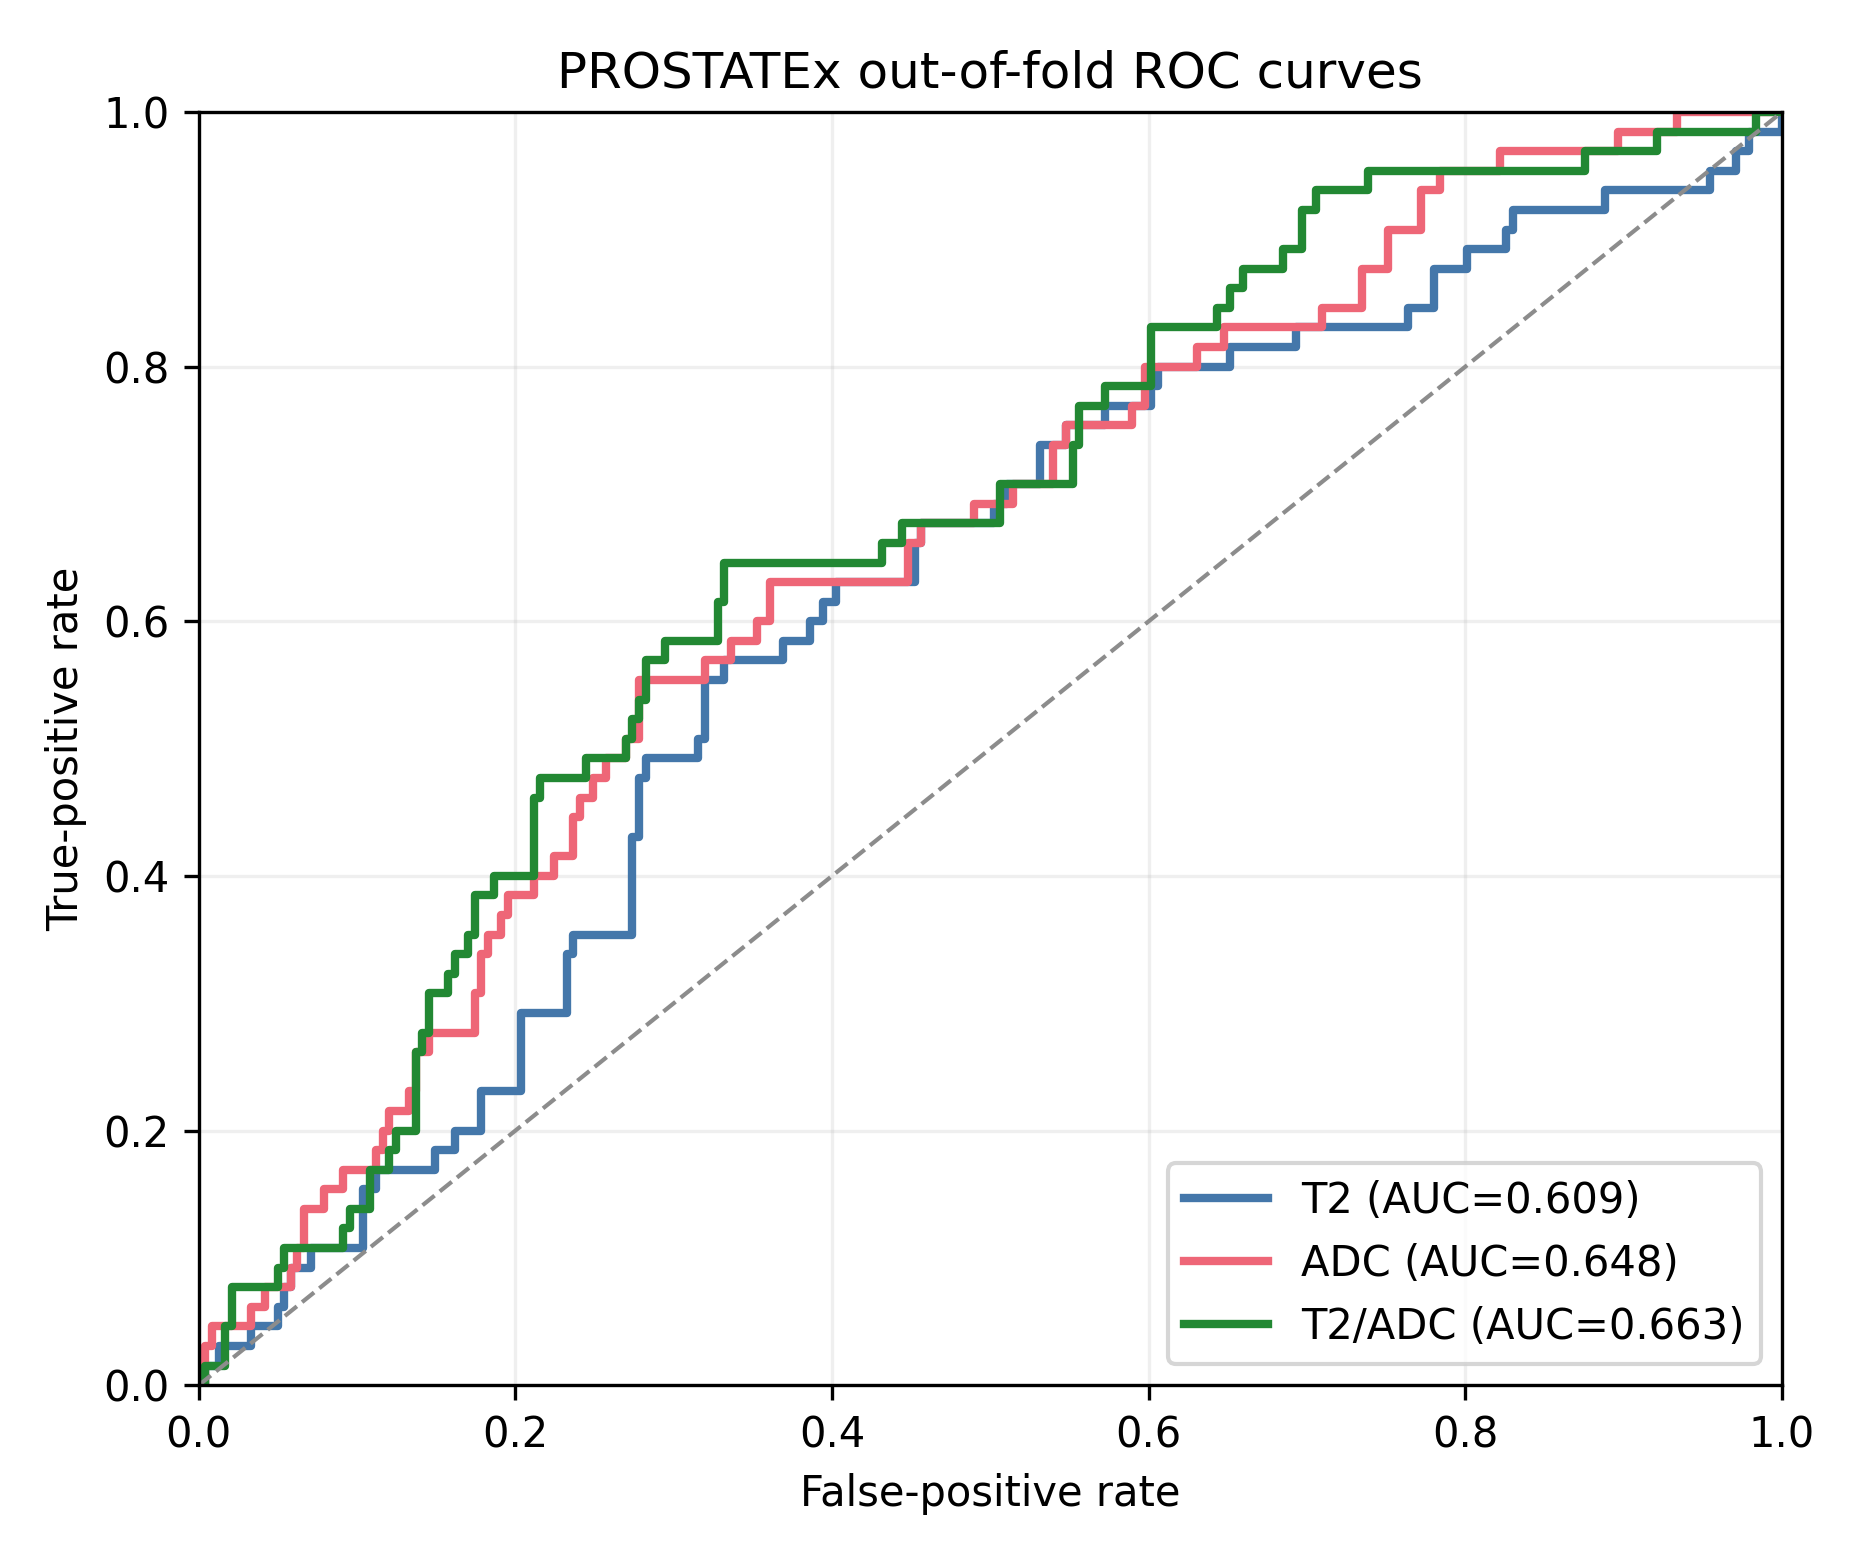
\includegraphics[width=\linewidth]{figures/prostatex_roc.png}
\end{minipage}\hfill
\begin{minipage}[t]{0.49\linewidth}
\centering
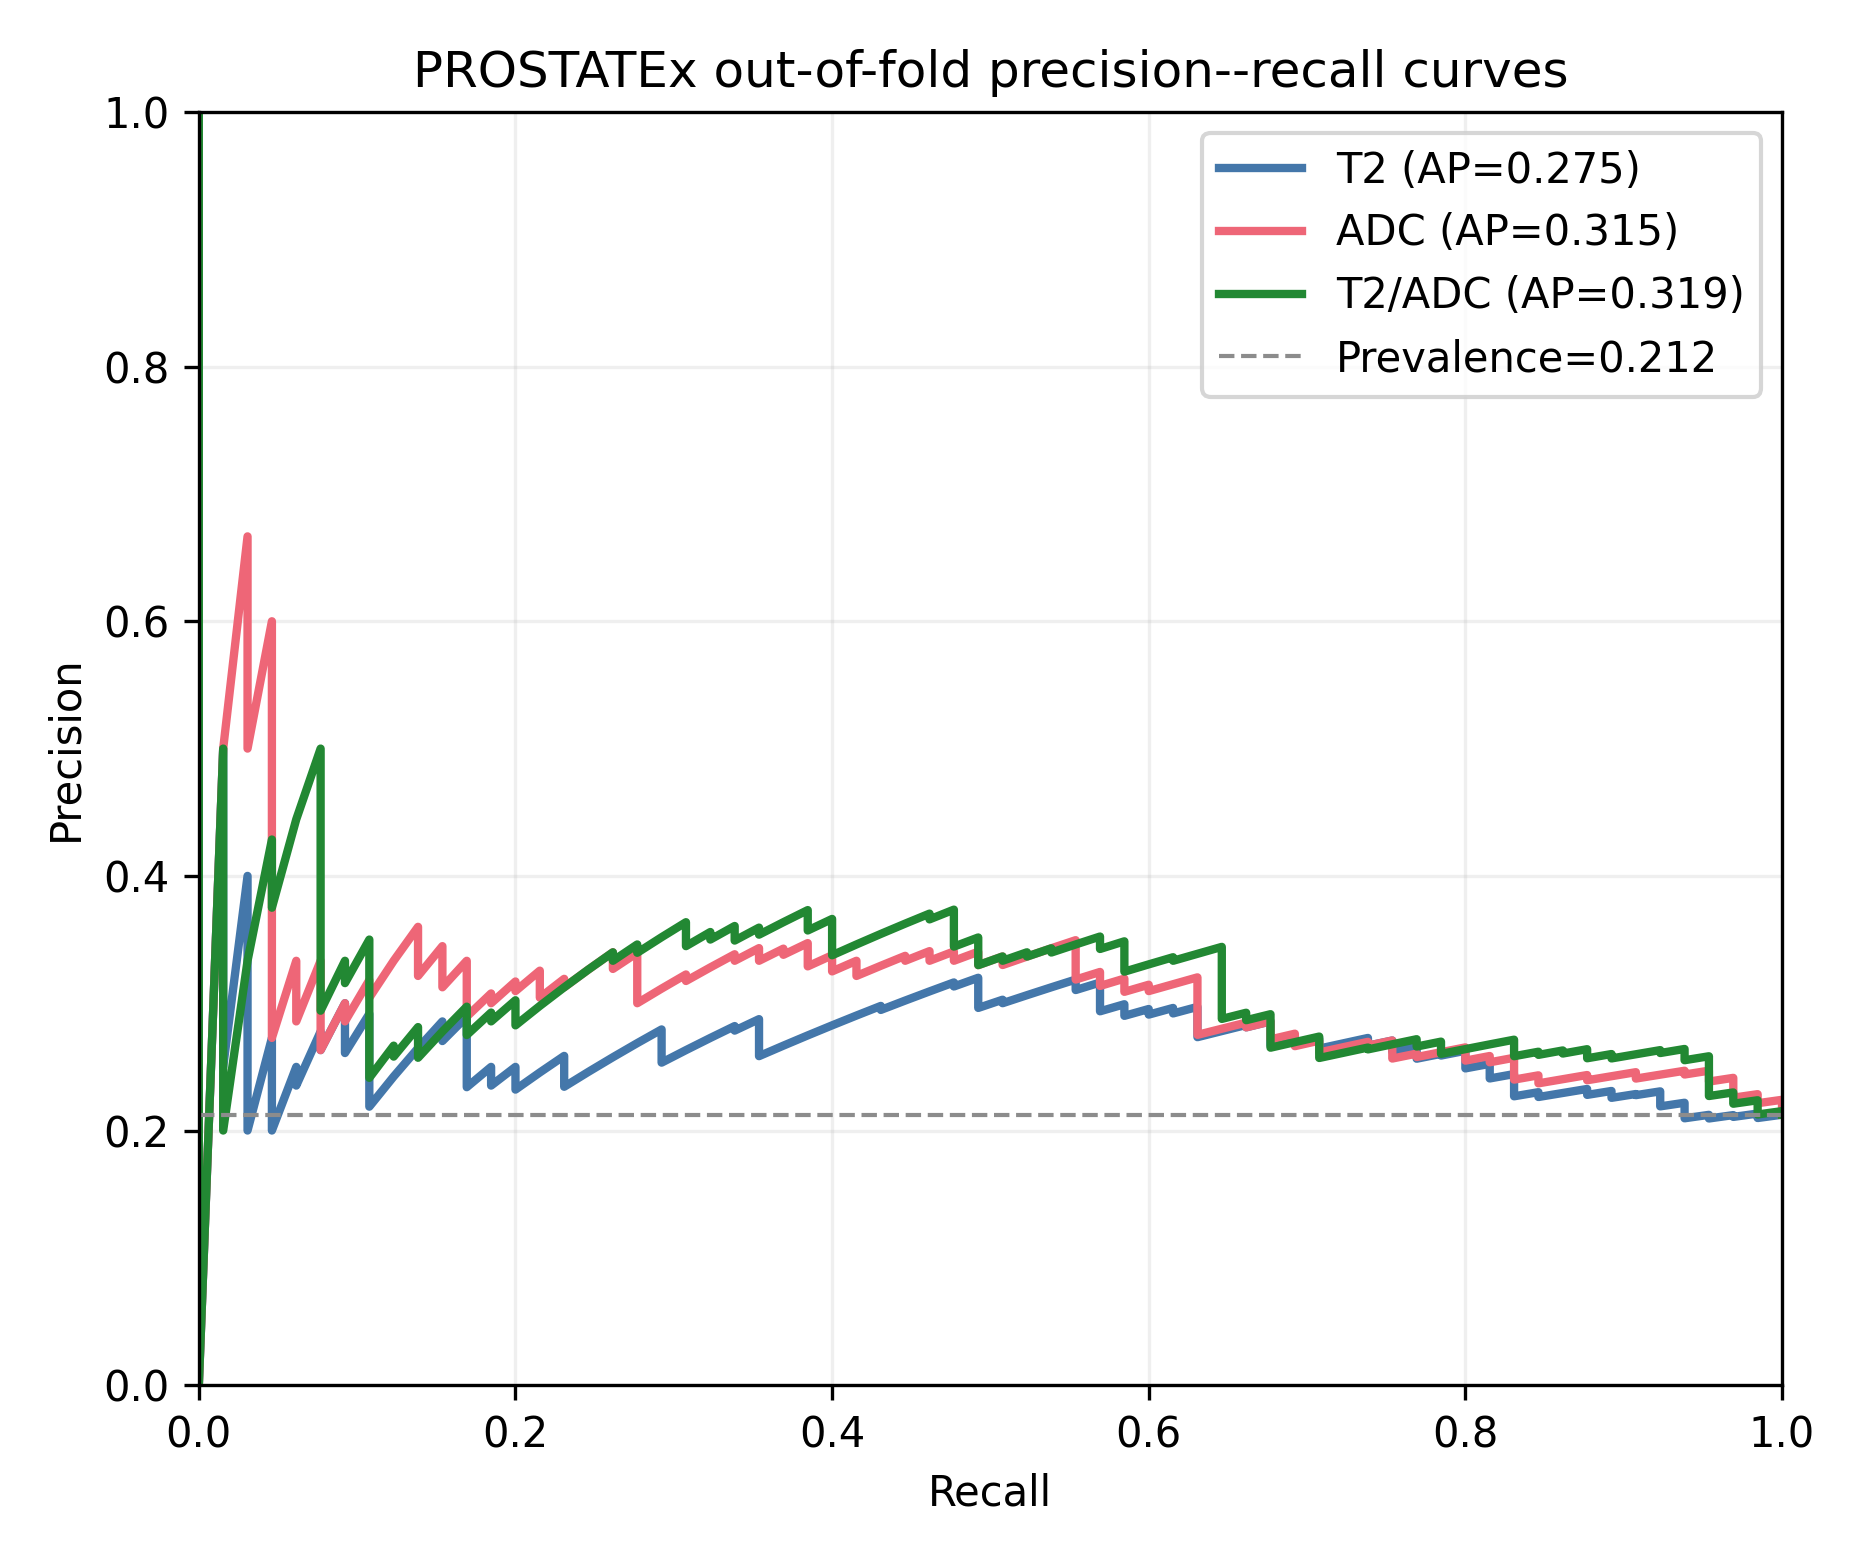
\includegraphics[width=\linewidth]{figures/prostatex_precision_recall.png}
\end{minipage}
\caption{Three-seed ensemble out-of-fold discrimination curves for the primary PROSTATEx fixed-CNN models. Left: receiver operating characteristic curves. Right: precision--recall curves, with the clinically significant finding prevalence shown as a dashed reference line.}
\label{fig:prostatex-curves}
\end{figure}

The five-bin calibration plot in Figure~\ref{fig:prostatex-calibration} shows that predicted probabilities are generally higher than observed event fractions, particularly in the upper displayed bins. Together with Brier scores of 0.2484, 0.2361, and 0.2355 for T2, ADC, and paired inputs, respectively, this indicates that the uncalibrated CNN scores should not be interpreted as clinical probabilities. Calibration is a distinct requirement from discrimination when predictions are intended to support decisions~\cite{van-calster-calibration}. The plot is descriptive because several bins contain few findings and no calibration confidence bands are reported.

\begin{figure}[htbp]
\centering
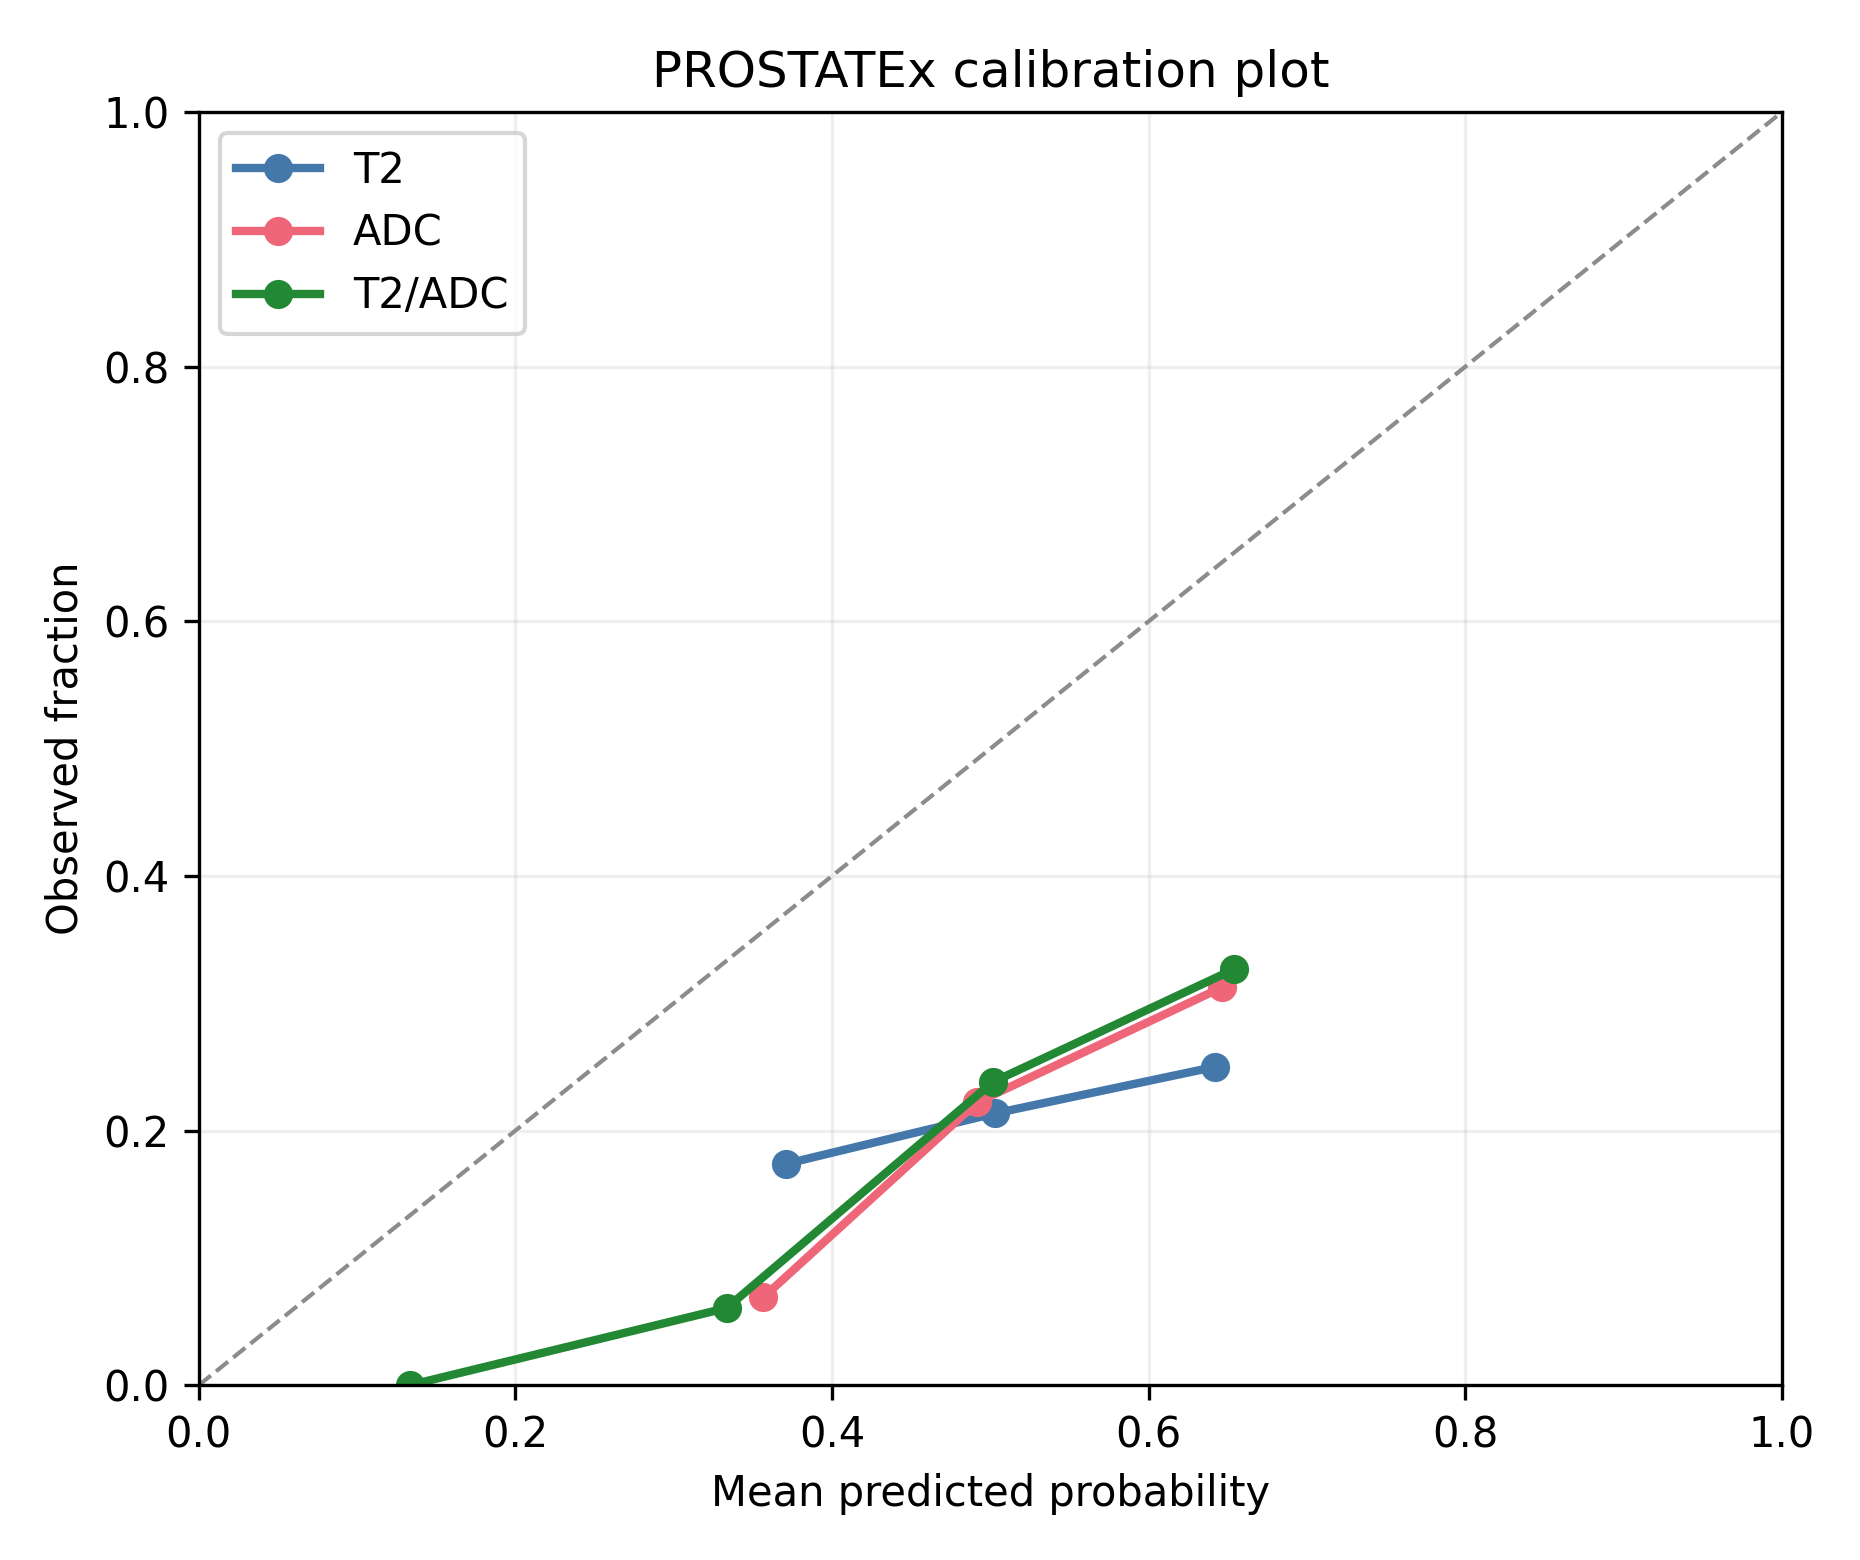
\includegraphics[width=0.62\linewidth]{figures/prostatex_calibration.png}
\caption{Five-bin descriptive calibration plot for the primary PROSTATEx fixed-CNN models. The dashed diagonal represents perfect calibration.}
\label{fig:prostatex-calibration}
\end{figure}

\subsection{Classical Baselines and Direct Comparisons}\label{sec:4.3}

Table~\ref{tab:5} reports the nine primary classical controls. Random-forest ADC has the highest classical AUC, 0.7205 (95\% CI 0.6516--0.7882), followed by random-forest paired T2/ADC at 0.7030 (0.6307--0.7729) and logistic ADC at 0.6883 (0.6179--0.7598). In a paired 10,000-replicate patient bootstrap, random-forest ADC exceeds the modality-matched ADC CNN by 0.0725 AUC (95\% CI 0.0084--0.1397). The other eight modality-matched classical-minus-CNN AUC intervals include zero. This comparison is exploratory and is not adjusted for the nine comparisons, but the results do not support a general advantage for the fixed CNN over simpler engineered-feature controls.

\begin{table}[htbp]
\centering
\scriptsize
\caption{Primary PROSTATEx classical controls using the same frozen patient-level folds. Confidence intervals use 2,000 patient-level bootstrap replicates. AP denotes average precision. Brier scores are reported for the raw model probabilities.}
\label{tab:5}
\resizebox{\linewidth}{!}{%
\begin{tabular}{@{}llrrr@{}}
\toprule
\textbf{Model} & \textbf{Input} & \textbf{AUC (95\% CI)} & \textbf{AP} & \textbf{Brier score} \\
\midrule
Logistic regression & T2 & 0.5963 (0.5089--0.6781) & 0.2917 & 0.2424 \\
Logistic regression & ADC & 0.6883 (0.6179--0.7598) & 0.4170 & 0.2208 \\
Logistic regression & T2/ADC & 0.6524 (0.5733--0.7285) & 0.3458 & 0.2245 \\
RBF SVM & T2 & 0.5868 (0.5056--0.6652) & 0.3009 & 0.1647 \\
RBF SVM & ADC & 0.6723 (0.5915--0.7432) & 0.3446 & 0.1591 \\
RBF SVM & T2/ADC & 0.6712 (0.5892--0.7491) & 0.3580 & 0.1589 \\
Random forest & T2 & 0.6270 (0.5544--0.7009) & 0.3200 & 0.1618 \\
Random forest & ADC & 0.7205 (0.6516--0.7882) & 0.3692 & 0.1541 \\
Random forest & T2/ADC & 0.7030 (0.6307--0.7729) & 0.3794 & 0.1552 \\
\bottomrule
\end{tabular}}
\end{table}

Figure~\ref{fig:prostatex-classical-auc} displays the same classical AUC estimates and patient-bootstrap intervals. The wide, overlapping intervals emphasize the limited precision of model rankings in this single cohort.

\begin{figure}[htbp]
\centering
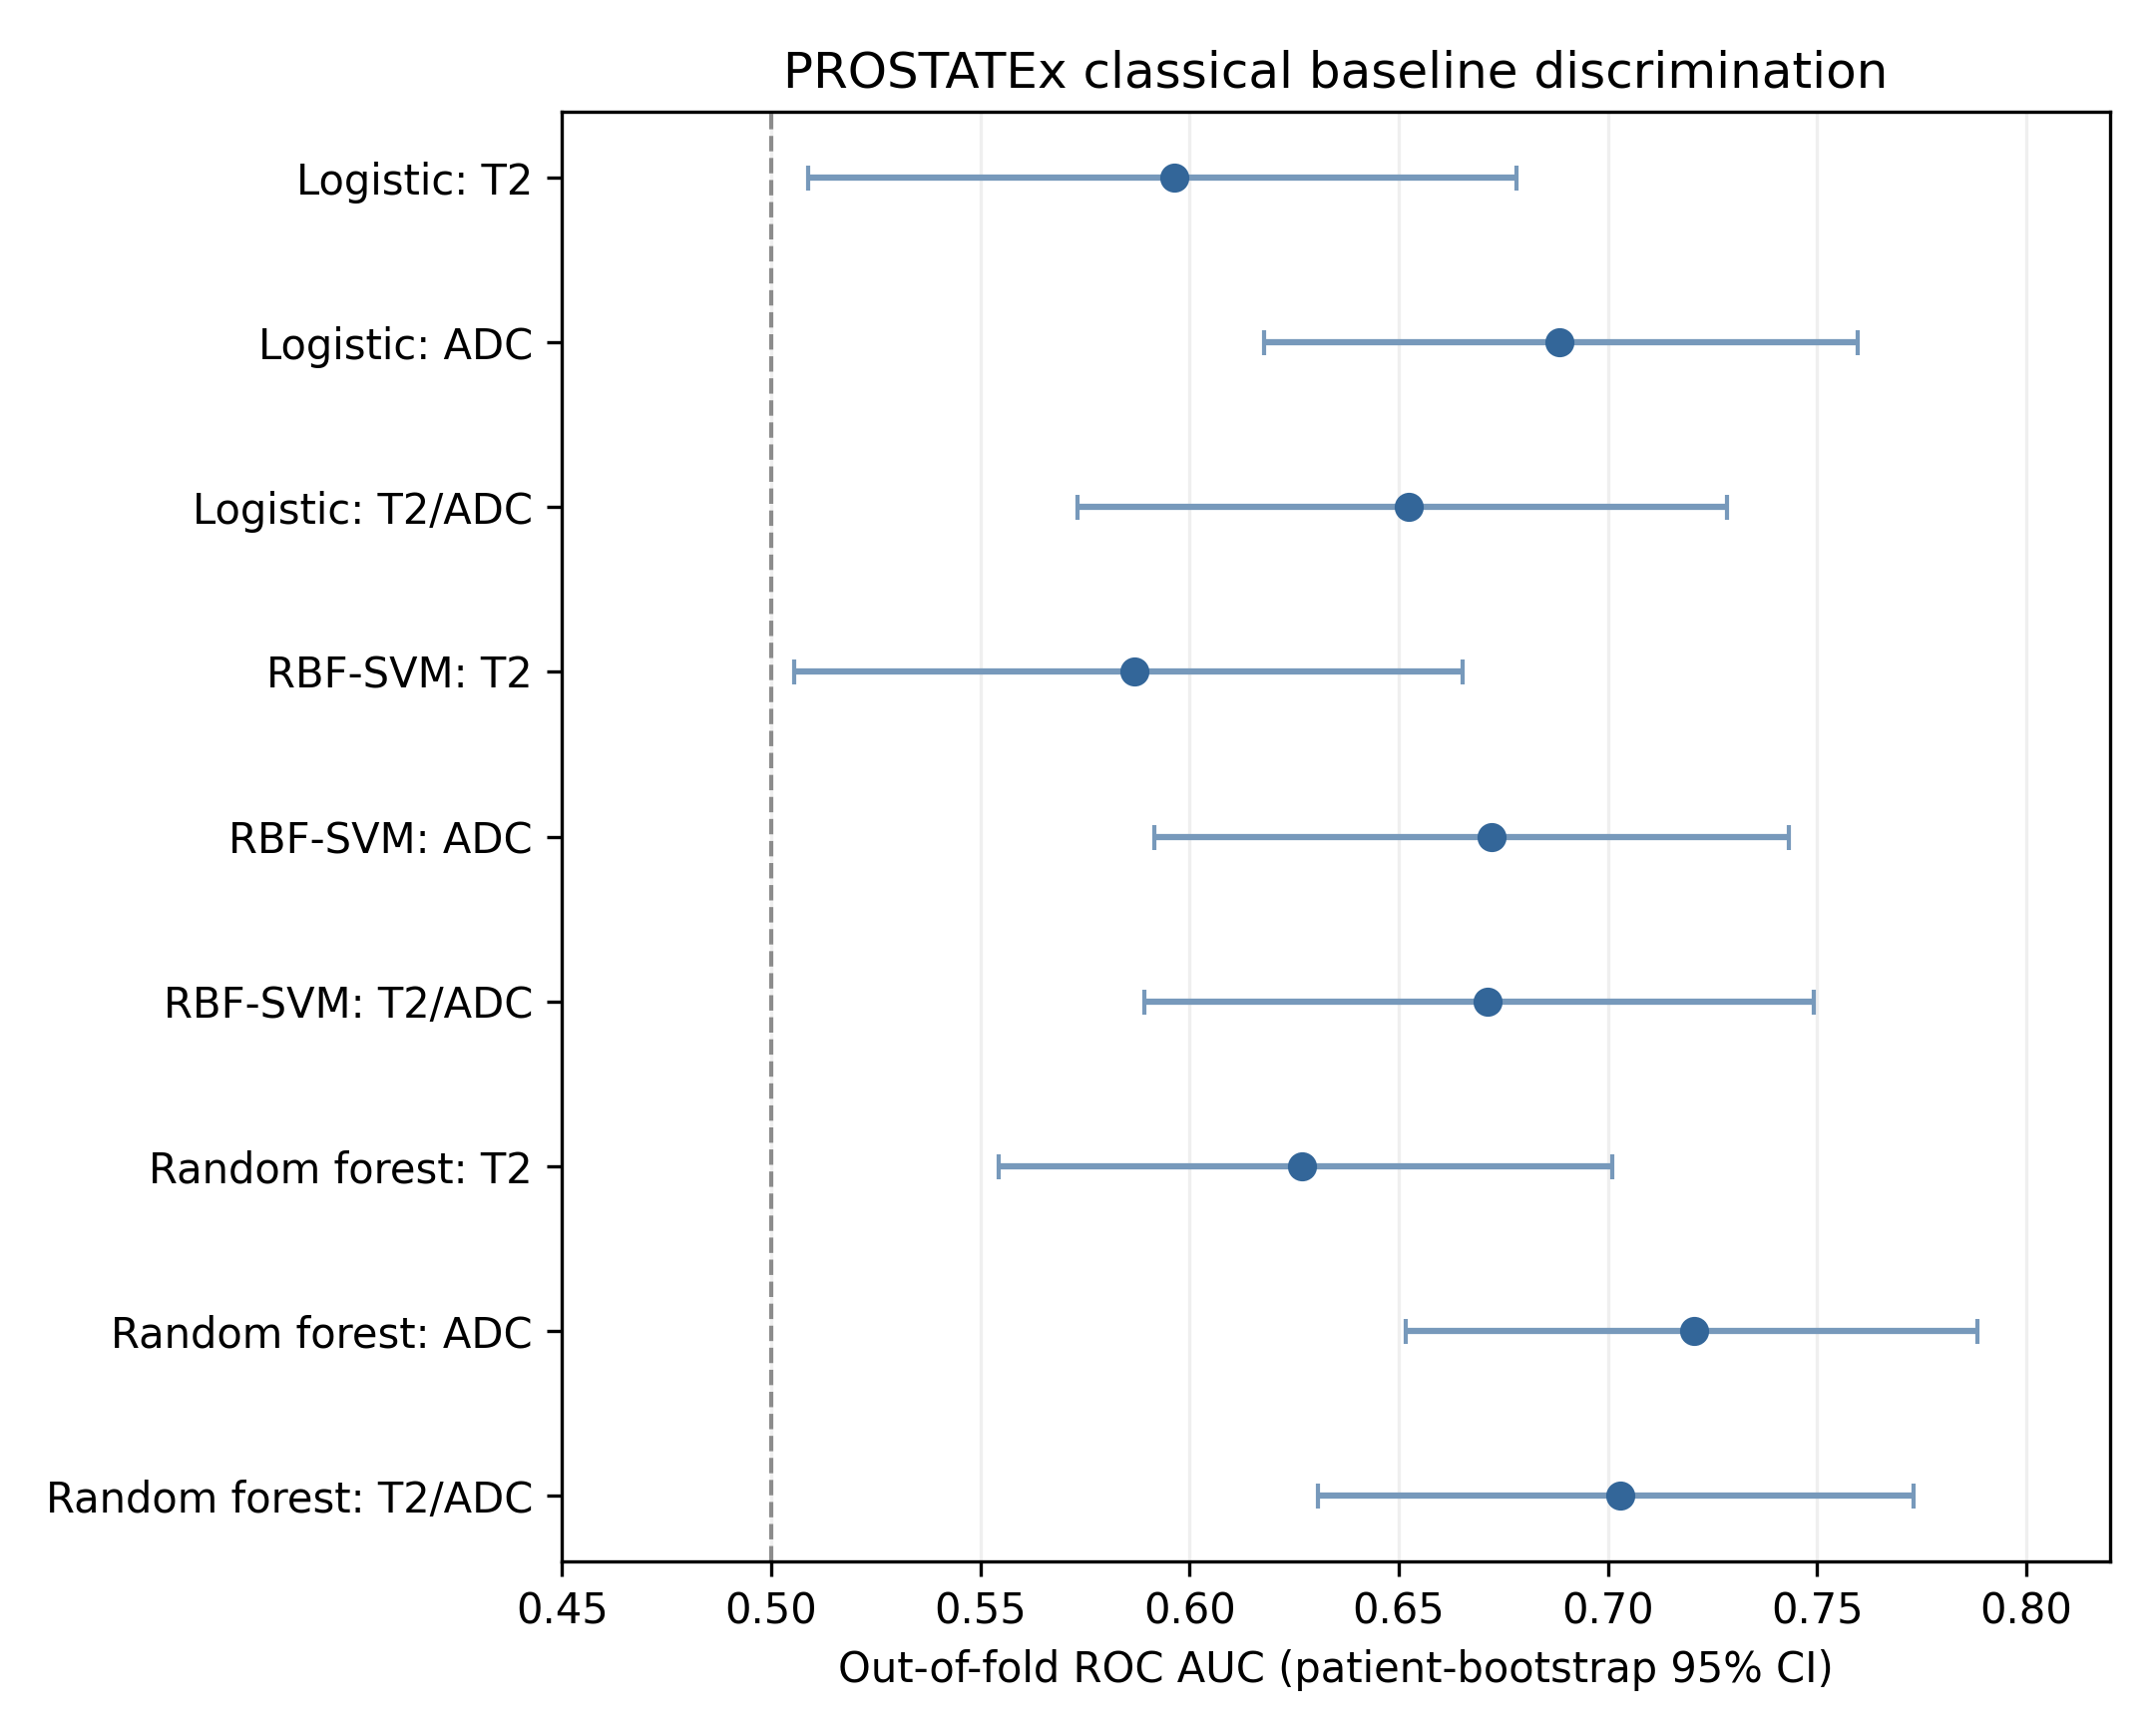
\includegraphics[width=0.78\linewidth]{figures/prostatex_classical_auc_forest.png}
\caption{Out-of-fold ROC AUC estimates for the nine primary classical PROSTATEx controls. Error bars are 95\% patient-bootstrap confidence intervals; the dashed line denotes chance discrimination.}
\label{fig:prostatex-classical-auc}
\end{figure}

Excluding the finding with limited native ADC support changes classical AUC by no more than 0.007 across the six repeated ADC and paired configurations, leaving the qualitative ranking unchanged. The high raw accuracy but near-chance balanced accuracy of several SVM and random-forest configurations also shows that a default 0.5 threshold is unsuitable under the observed class imbalance. Discrimination, threshold selection, and calibration should therefore be assessed separately.

\section{Discussion}\label{sec:5}

\subsection{Principal Findings}\label{sec:5.1}

The central finding is that reproducible patient-level evaluation was feasible, but no tested model achieved sufficiently strong or precise performance to support clinical use. Among the fixed CNNs, paired T2/ADC produced the highest observed AUC (0.6634), followed by ADC (0.6479) and T2 (0.6086). However, the paired patient-bootstrap intervals for the CNN AUC differences included zero, so the apparent ordering does not establish that combining T2 and ADC improves discrimination. The sensitivity analysis excluding the single finding with limited native ADC support changed all repeated AUC estimates by less than 0.01 and did not alter the qualitative ranking.

The best observed primary result was the random-forest ADC model, with an AUC of 0.7205 (95\% CI 0.6516--0.7882). Its AUC exceeded that of the modality-matched ADC CNN by 0.0725 in the exploratory paired bootstrap (95\% CI 0.0084--0.1397). This comparison was not adjusted for multiplicity and should therefore be interpreted as hypothesis-generating. The other eight modality-matched classical-versus-CNN AUC intervals included zero. Collectively, these findings do not support a general advantage for convolutional modeling in this cohort and emphasize the value of directly matched classical controls.

\subsection{Modality and Model Comparisons}\label{sec:5.2}

ADC was the strongest single input for logistic regression and random forest, while paired input produced only a small, uncertain improvement over ADC for the fixed CNN and a small decrease for random forest. T2 alone was consistently weaker. These results suggest that diffusion-derived contrast carried useful discriminatory information in the extracted neighborhoods, but they do not show that the selected ADC values had verified quantitative physical meaning. The absence of an established paired-input advantage may reflect limited sample size, imperfect cross-sequence alignment, the use of local two-dimensional patches, or insufficient model capacity to exploit complementary anatomy.

Published PROSTATEx results provide context rather than direct benchmarks. Volumetric CNN and radiomics studies have reported stronger discrimination using additional sequences, manual contours, anatomical information, or the original challenge test protocol~\cite{mehrtash-prostatex,kwon-prostatex}. Differences in cohort composition, image inputs, annotation, tuning, and evaluation design prevent attribution of the performance gap to model architecture alone. The present comparisons are strongest internally because every model used the same retained findings, outer folds, and out-of-fold evaluation framework.

\subsection{Thresholding and Calibration}\label{sec:5.3}

Metric rankings were not identical. Logistic regression on ADC had the highest average precision among the classical controls, whereas random-forest ADC had the highest AUC and random-forest paired input had a slightly higher average precision than random-forest ADC. Several support-vector-machine and random-forest configurations also combined high raw accuracy with balanced accuracy near chance at the default 0.5 threshold. This pattern reflects class imbalance and probability-scale behavior rather than reliable operating-point performance. The CNN Brier scores and descriptive calibration analyses likewise indicated overprediction. Any future threshold must therefore be selected within training data for a prespecified clinical objective and evaluated independently; a default probability cutoff should not be treated as clinically meaningful.

\subsection{Reproducibility Strengths}\label{sec:5.4}

The main strength of this study is procedural rather than predictive. Eligibility rules, series selection, paired-patch construction, patient-level folds, model grids, and sensitivity handling were frozen and archived. Patient identity was preserved during outer-fold testing and bootstrap resampling, preventing findings from the same patient from being treated as independent observations. CNN and classical results were reconstructed from complete out-of-fold prediction tables, and the full run archives include fold-level outputs and model artifacts. These controls make the reported estimates auditable and provide a stable baseline for subsequent development.

\subsection{Limitations}\label{sec:5.5}

The study uses one public cohort without external validation, so transportability across institutions, scanners, acquisition protocols, and patient populations is unknown. Image review was technical and label-hidden rather than a qualified diagnostic assessment. ADC physical units were not independently verified, and the models used coordinate-centered patches without lesion, gland, or zonal segmentation. The contents of the finding and imaging CSV files were hash-tracked, but the provenance of the original label-file container was not independently established. The fixed CNNs and deterministic intensity summaries were intentionally compact and do not represent optimized three-dimensional networks or validated radiomics pipelines. Hyperparameter searches differed by model family and were not equal-compute comparisons.

The paired comparisons were exploratory and unadjusted for multiplicity. Bootstrap intervals quantify patient-resampling uncertainty conditional on the frozen dataset and analysis pipeline; they do not capture uncertainty from alternative series selection, preprocessing, architecture design, or reference-standard construction. Threshold-dependent metrics are sensitive to class prevalence and calibration, and no decision-curve or prospective clinical-impact analysis was performed. The results should consequently be interpreted as reproducible computational benchmarks, not evidence of diagnostic efficacy or clinical utility.

\section{Conclusion}\label{sec:6}

This study establishes an auditable patient-level pipeline for classifying clinically significant prostate cancer findings from paired T2-weighted and ADC MRI patches in PROSTATEx. Fixed CNN AUCs ranged from 0.6086 to 0.6634, while the strongest observed classical control was random-forest ADC with an AUC of 0.7205. Its exploratory paired advantage over the ADC CNN was modest and unadjusted for multiple comparisons, and no consistent benefit from paired T2/ADC input was established. The principal contribution is therefore a reproducible benchmark with complete out-of-fold artifacts, not a clinically validated classifier. External validation, verified image semantics, qualified review, stronger lesion-aware models, and prespecified calibration and operating-point assessment are required before stronger claims are justified.

\section{Future Work}\label{sec:7}

\subsection{External Validation and Image Semantics}\label{sec:7.1}

The highest priority is evaluation on an independent prostate MRI cohort using a protocol frozen before outcome analysis. Dataset selection should reflect current benchmark relevance and provide sufficient metadata to verify sequence identity, ADC units, acquisition characteristics, and reference-standard provenance. Qualified reviewers should assess image quality and localization while blinded to model predictions, and exclusion or support criteria should be defined before performance is examined.

\subsection{Stronger Imaging Models and Inputs}\label{sec:7.2}

Subsequent experiments should compare validated radiomics, transfer learning, three-dimensional or multi-slice networks, and lesion-, gland-, or zone-aware inputs under the same patient partitions and matched tuning budgets. Registration strategies and the incremental value of T2, ADC, high-b-value diffusion imaging, and other clinically available sequences should be tested explicitly. More complex augmentation or automated architecture search should be considered only after strong conventional baselines and leakage-resistant validation are established.

\subsection{Calibration and Clinical Evaluation}\label{sec:7.3}

Future work should fit calibration procedures using training and validation patients only, prespecify clinically relevant operating points, and report sensitivity, specificity, predictive values, and uncertainty on untouched external data. Decision-curve analysis or another explicit utility framework would be needed to determine whether predictions improve decisions relative to established clinical strategies. Prospective evaluation would remain necessary before deployment.

\section*{Data and Code Availability Statement}

PROSTATEx is publicly available from The Cancer Imaging Archive~\cite{prostatex}; source images are not redistributed with this manuscript. The study artifacts comprise the frozen eligibility and fold records, patch-generation and modeling scripts, 75 CNN run outputs, three-seed out-of-fold CNN prediction tables, 75 classical run outputs, classical out-of-fold prediction tables, and summary metrics. Complete archive filenames, sizes, SHA-256 checksums, and integrity results are recorded in the accompanying audit manifests. A public repository or permanent archival record is required before the code and generated artifacts can be described as publicly available.

% Bibliographic initials, title punctuation, and DOI/URL hyphens are intentional.
% chktex-file 8
% chktex-file 12
% chktex-file 13
% chktex-file 38
\begin{thebibliography}{99}

\bibitem{pirads-v21} B. Turkbey, A. B. Rosenkrantz, M. A. Haider, et al., ``Prostate Imaging Reporting and Data System Version 2.1: 2019 update of Prostate Imaging Reporting and Data System Version 2,'' \emph{European Urology}, vol. 76, no. 3, pp. 340--351, 2019, doi: \url{https://doi.org/10.1016/j.eururo.2019.02.033}.

\bibitem{pirads-pathway} A. R. Padhani, J. Barentsz, G. Villeirs, et al., ``PI-RADS Steering Committee: The PI-RADS multiparametric MRI and MRI-directed biopsy pathway,'' \emph{Radiology}, vol. 292, no. 2, pp. 464--474, 2019, doi: \url{https://doi.org/10.1148/radiol.2019182946}.

\bibitem{selection-bias} G. C. Cawley and N. L. C. Talbot, ``On over-fitting in model selection and subsequent selection bias in performance evaluation,'' \emph{Journal of Machine Learning Research}, vol. 11, pp. 2079--2107, 2010. \url{https://www.jmlr.org/papers/v11/cawley10a.html}.

\bibitem{prostatex} G. Litjens, O. Debats, J. Barentsz, N. Karssemeijer, and H. Huisman, ``SPIE-AAPM PROSTATEx Challenge Data (Version 2),'' The Cancer Imaging Archive, 2017, dataset, doi: \url{https://doi.org/10.7937/K9TCIA.2017.MURS5CL}. Collection status consulted September 11, 2026.

\bibitem{armato-prostatex} S. G. Armato III, H. Huisman, K. Drukker, et al., ``PROSTATEx Challenges for computerized classification of prostate lesions from multiparametric magnetic resonance images,'' \emph{Journal of Medical Imaging}, vol. 5, no. 4, article 044501, 2018, doi: \url{https://doi.org/10.1117/1.JMI.5.4.044501}.

\bibitem{mehrtash-prostatex} A. Mehrtash, A. Sedghi, M. Ghafoorian, et al., ``Classification of clinical significance of MRI prostate findings using 3D convolutional neural networks,'' \emph{Proceedings of SPIE Medical Imaging}, vol. 10134, article 101342A, 2017, doi: \url{https://doi.org/10.1117/12.2277123}.

\bibitem{schelb-pirads} P. Schelb, S. Kohl, J. P. Radtke, et al., ``Classification of cancer at prostate MRI: Deep learning versus clinical PI-RADS assessment,'' \emph{Radiology}, vol. 293, no. 3, pp. 607--617, 2019, doi: \url{https://doi.org/10.1148/radiol.2019190938}.

\bibitem{kwon-prostatex} D. Kwon, I. M. Reis, A. L. Breto, et al., ``Classification of suspicious lesions on prostate multiparametric MRI using machine learning,'' \emph{Journal of Medical Imaging}, vol. 5, no. 3, article 034502, 2018, doi: \url{https://doi.org/10.1117/1.JMI.5.3.034502}.

\bibitem{castillo-validation} J. M. Castillo Tovar, M. Arif, M. P. A. Starmans, et al., ``Classification of clinically significant prostate cancer on multi-parametric MRI: A validation study comparing deep learning and radiomics,'' \emph{Cancers}, vol. 14, no. 1, article 12, 2022, doi: \url{https://doi.org/10.3390/cancers14010012}.

\bibitem{picai-confirmatory} A. Saha, J. S. Bosma, J. J. Twilt, et al., ``Artificial intelligence and radiologists in prostate cancer detection on MRI (PI-CAI): An international, paired, non-inferiority, confirmatory study,'' \emph{The Lancet Oncology}, vol. 25, no. 7, pp. 879--887, 2024, doi: \url{https://doi.org/10.1016/S1470-2045(24)00220-1}.

\bibitem{claim} J. Mongan, L. Moy, and C. E. Kahn Jr., ``Checklist for Artificial Intelligence in Medical Imaging (CLAIM): A guide for authors and reviewers,'' \emph{Radiology: Artificial Intelligence}, vol. 2, no. 2, article e200029, 2020, doi: \url{https://doi.org/10.1148/ryai.2020200029}.

\bibitem{tripod-ai} G. S. Collins, K. G. M. Moons, P. Dhiman, et al., ``TRIPOD+AI statement: Updated guidance for reporting clinical prediction models that use regression or machine learning methods,'' \emph{BMJ}, vol. 385, article e078378, 2024, doi: \url{https://doi.org/10.1136/bmj-2023-078378}.

\bibitem{van-calster-calibration} B. Van Calster, D. J. McLernon, M. van Smeden, et al., ``Calibration: The Achilles heel of predictive analytics,'' \emph{BMC Medicine}, vol. 17, article 230, 2019, doi: \url{https://doi.org/10.1186/s12916-019-1466-7}.

\end{thebibliography}
\end{document}